\documentclass{paper}
%\hyphenation{Post-Script}
\usepackage[authoryear]{natbib}
%\bibliographystyle{plainnat}
\usepackage{fma2014}

\usepackage{graphicx}
%\usepackage{amssymb}

%\usepackage{xcolor}
%\usepackage{hyperref} % Apparemment pas compatible avec le style AES !!
\usepackage{url}
\usepackage[utf8]{inputenc}
\usepackage[T1]{fontenc}
%\usepackage{enumitem}
%\setlist{nosep}

%\setlength{\parskip}{0pt}

%----------
%  Header
%----------


% first the title is needed
\title{An open web audio platform for ethnomusicological sound archives management and automatic analysis}

% a short form should be given in case it is too long for the running head
%\shorttitle{Telemeta : open web audio platform for sound archives}

\threeauthors
  {Thomas Fillon} {
    PARISSON / LAM, \\
Institut Jean Le Rond d'Alembert, \\
     UPMC Univ. Paris 06, \\
  UMR CNRS 7190\\
   %PARISSON\\
 {\tt  thomas.fillon@parisson.com}}
 %\href{http://www.parisson.com}{PARISSON}, 16 rue Jacques Louvel-Tessier 75010 Paris, France
 %\url{{thomas.fillon,guillaume.pellerin}@parisson.com}}
  {Guillaume Pellerin, Paul Brossier} {
    PARISSON \\
16 rue Jacques Louvel-Tessier \\
 Paris, France\\ \vspace{0.3cm}
    {\tt guillaume.pellerin@parisson.com}}
  {Jos{\'e}phine Simonnot} {CREM, LESC, UMR CNRS 7186\\MAE, Université Paris Ouest\\ Nanterre La Défense
{\tt %josephine.simonnot@mae.u-paris10.fr
}\thanks{This work is partly supported by a grant from the french National Research Agency (ANR) with reference ANR-12-CORD-0022.}\vspace{0.7cm}}



\begin{document}
%
\maketitle
%
\begin{abstract}
Since 2007, ethnomusicologist and engineers have joint their effort to develop a scalable and collaborative web platform for management of and access to digital sound archives. This platform has been deployed since 2011 and hold the archives of the \emph{Center for Research in Ethnomusicology}, which is the most important collection in Europe.
This web platform is based on \emph{Telemeta}, an open-source web audio framework dedicated to digital sound archives secure storing, indexing and publishing. It focuses on the enhanced and collaborative user-experience in accessing audio items and their associated metadata and on the possibility for the expert users to further enrich those metadata.

 Telemeta architecture relies on \emph{TimeSide}, an open audio processing framework written in Python which provides decoding,  encoding and streaming methods for various formats together with a smart embeddable HTML audio player. TimeSide also includes a set of audio analysis plugins and additionally wraps several audio features extraction libraries to provide automatic annotation, segmentation and musicological analysis.

\end{abstract}

\section{Introduction}\label{sec:intro}

 In social sciences like anthropology and linguistics, researchers have to work on multiple types of multimedia documents such as photos, videos, sound recordings or databases. The need to easily access, visualize and annotate such materials can be problematic given their diverse formats, sources and given their chronological nature.
  %With this in mind, some laboratories\footnote{The Research Center on Ethnomusicology (CREM), the Musical Acoustics Laboratory (LAM, UMR 7190) and the sound archives of the Mediterranean House of Human Sciences (MMHS)} involved in ethnomusicological research have been working together on that issue.

 In the context of ethnomusicological research, the Research Center on Ethnomusicology (CREM) and Parisson, a company specialized in big music data projects, have been developing an innovative, collaborative and interdisciplinary open-source web-based multimedia platform since 2007. 

 This platform, \emph{Telemeta} is designed to fit the professional requirements from both sound archivists, researchers and musicians to work together on big music data. The first prototype of this platform has been online since 2010 and is now fully operational and used on a daily basis for ethnomusicological studies since 2011. A description of theses archives and some use cases are given in Section~\ref{sec:archives-CREM}.

The benefit of this collaborative platform for ethnomusicological research has been described in several publications \citep{Simmonot_IASA_2011, Julien_IASA_2011, Simonnot_ICTM_2014}.

Recently, an open-source audio analysis framework, TimeSide, has been developed to bring automatic music analysis capabilities to the web platform and thus have turned Telemeta into a complete resource for \emph{Computational Ethnomusicology} \citep{Tzanetakis_2007_JIMS, Gomez_JNMR_2013}.
%Section~\ref{sec:TimeSide} 

 \section{The Telemeta platform}\label{sec:Telemeta}
 \subsection{Web audio content management features and architecture}
The primary purpose of the project is to provide the ethnomusicological communities with a scalable system to access, preserve and share audio research materials together with their associated metadata, as these data provide key information on the context and significance of the recording. Telemeta\footnote{http://telemeta.org}, as a free and open source\footnote{Telemeta code is available under the CeCILL Free Software License Agreement}, is a unique scalable web audio platform for backuping, indexing, transcoding, analyzing, sharing and visualizing any digital audio or video file in accordance with open web standards.

The time-based nature of such audio-visual materials and some associated metadata as annotations raises issues of access and visualization at a large scales. Easy and on demand access to these data, as you listen to the recording, represents a significant improvement.

An overview of the Telemeta's web interface is illustrated in Figure~\ref{fig:Telemeta}.
\begin{figure}
   \centering
   \fbox{\includegraphics[width=0.97\linewidth]{img/telemeta_screenshot_en.png}}
   \caption[1]{Screenshot excerpt of the Telemeta web interface}
    \label{fig:Telemeta}
 \end{figure}
Its flexible and streaming safe architecture is represented in Figure~\ref{fig:TM_arch}.
\begin{figure*}[htbp]
  \centering
  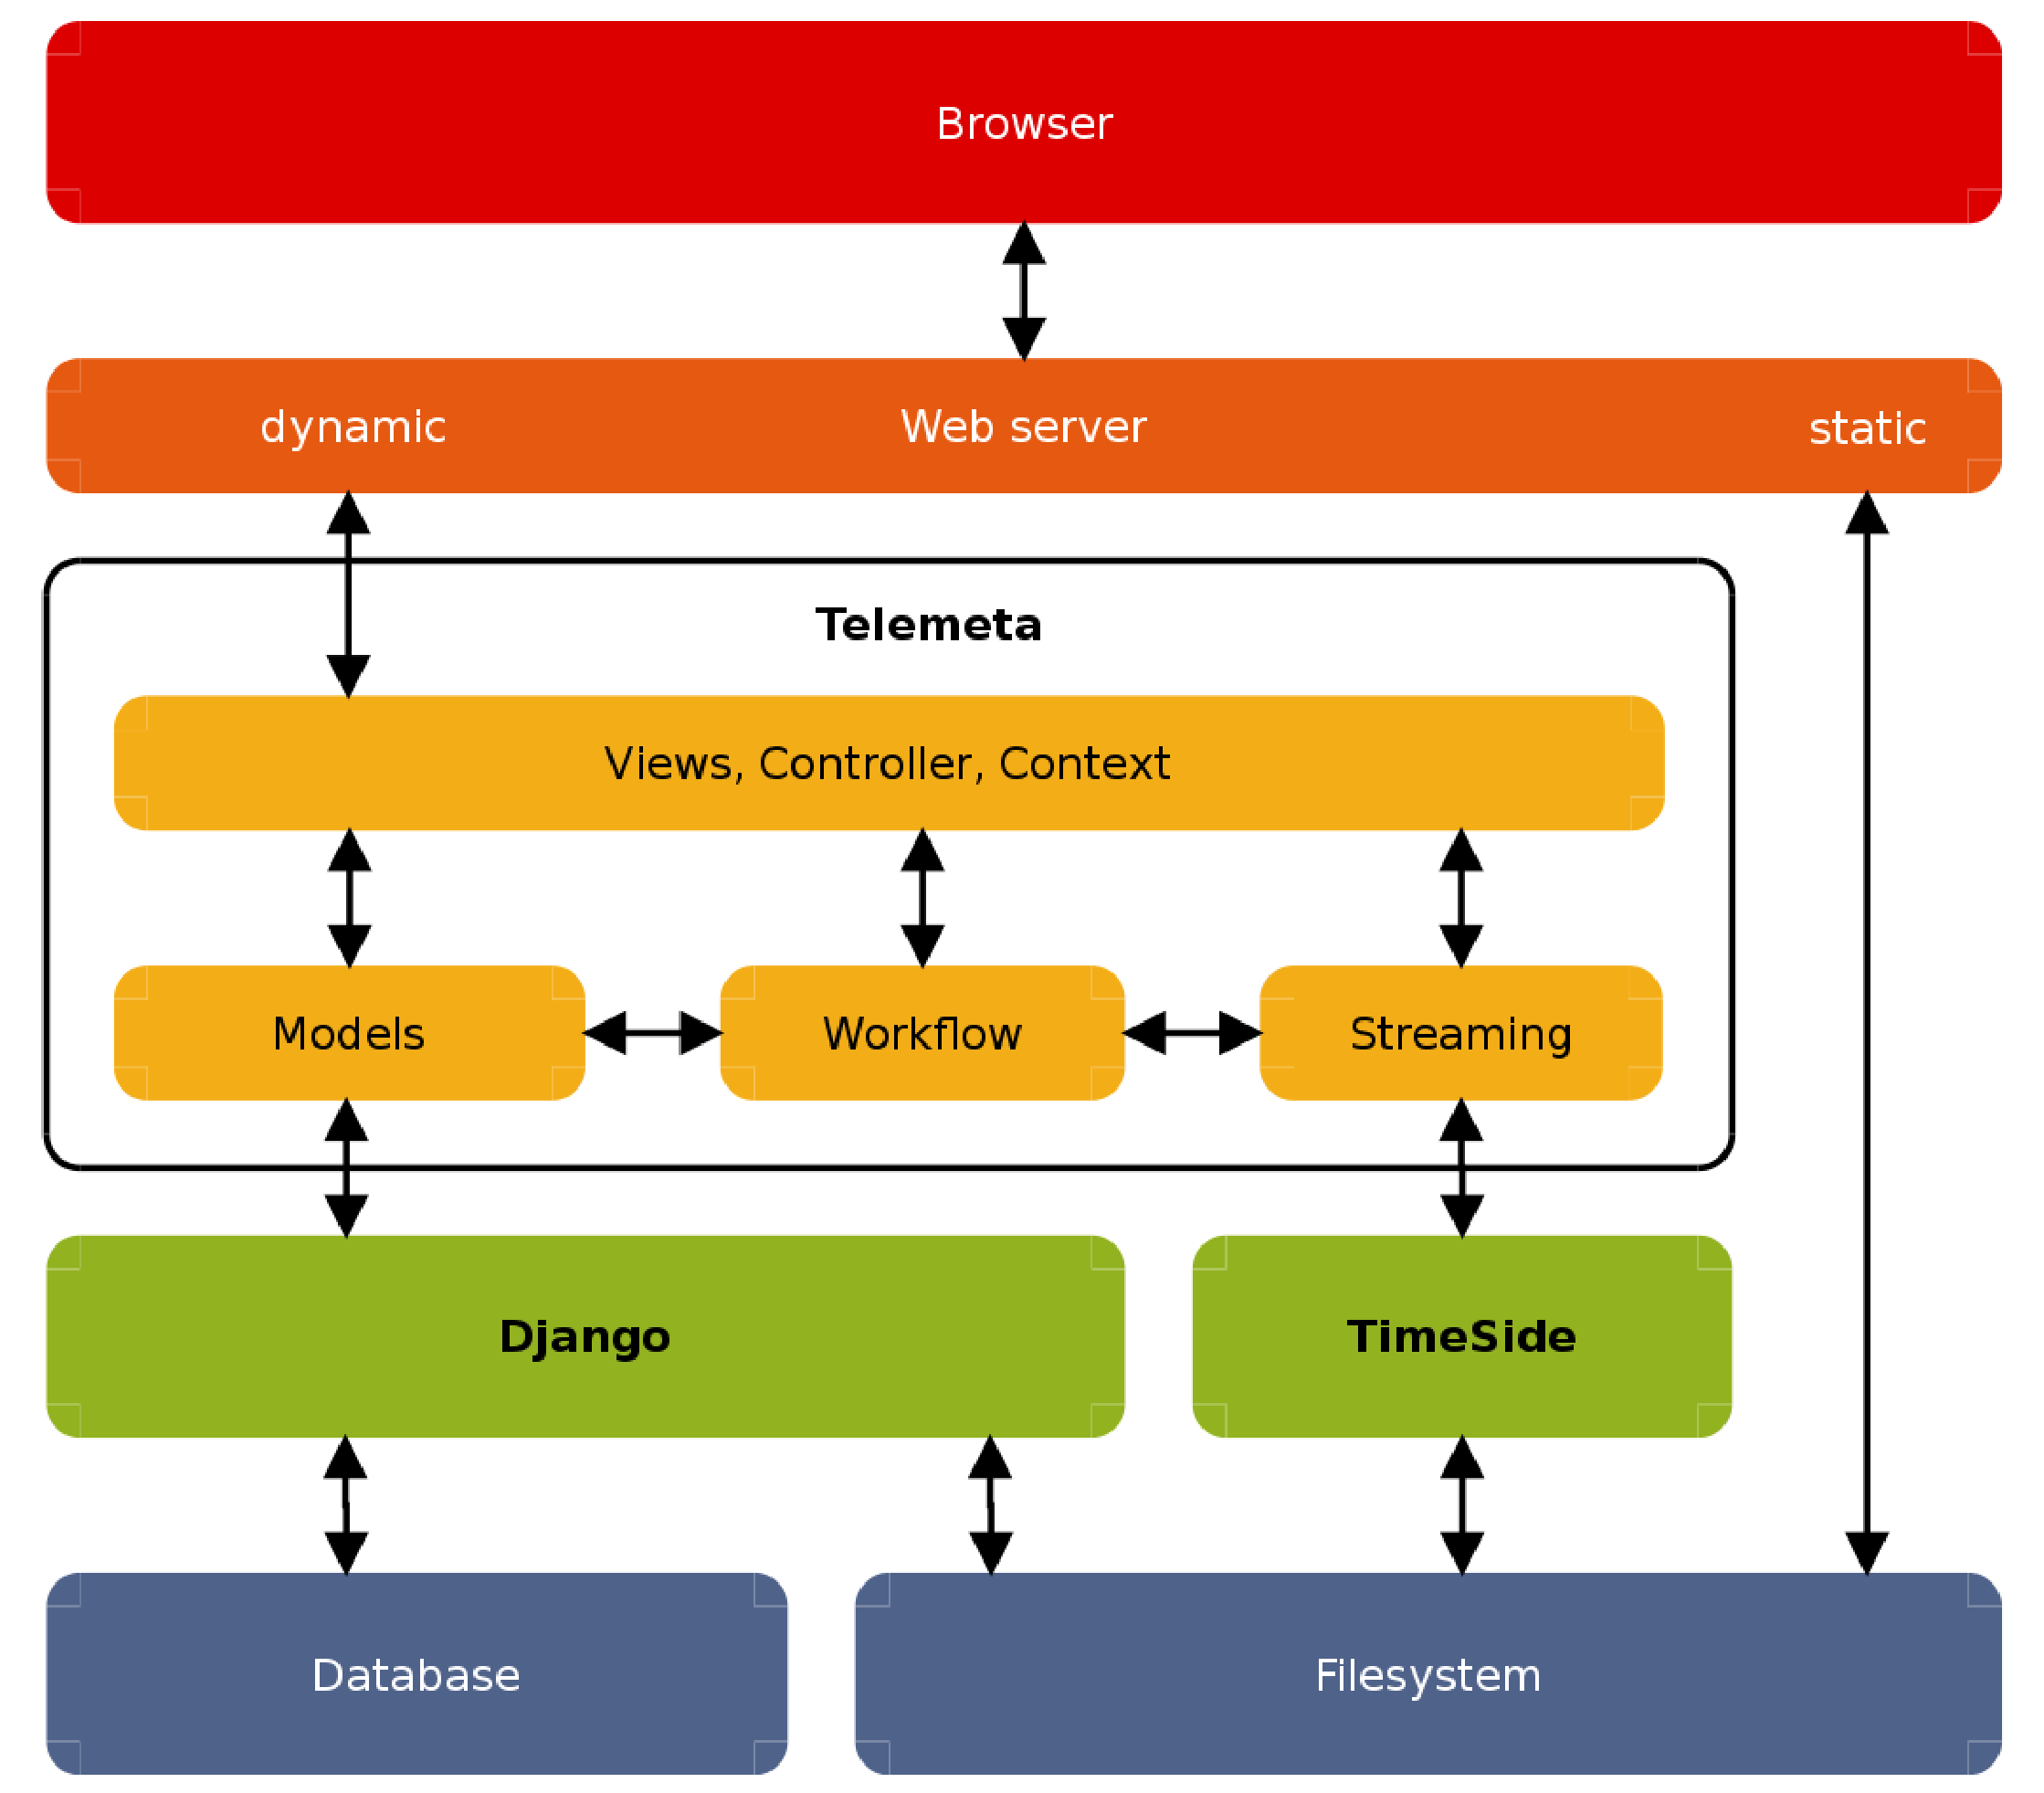
\includegraphics[width=0.5\linewidth]{img/TM_arch.pdf}
  \caption{Telemeta architecture}\label{fig:TM_arch}
\end{figure*}

The main features of \emph{Telemeta} are:

      \begin{itemize}
      \item Pure HTML5 web user interface including dynamical forms
      \item On the fly audio analyzing, transcoding and metadata
        embedding in various formats
      \item Social editing with semantic ontologies, smart workflows,
        realtime tools, human or automatic annotations and
        segmentations
      \item User management with individual desk, playlists, profiles
        and group access rights
      \item High level search engine (geolocation, instruments, ethnic groups, etc...)
      \item Data providers : DublinCore, OAI-PMH, RSS, XML, JSON and other 
      \item Multi-language support (now english and french)
      \end{itemize}

Beside database management, the audio support is mainly provided through an external component, TimeSide, which is described in Section~\ref{sec:TimeSide}.
\defcitealias{DublinCore}{Papier I}

\subsection{Metadata}\label{sec:metadata}
In addition to the audio data, an efficient and dynamic management of the associated metadata is also required. Consulting metadata provide both an exhaustive access to valuable information about the source of the data and to the related work of peer researchers. 
Dynamically handling metadata in a collaborative manner optimises the continuous process of knowledge gathering and enrichment of the materials in the database.  
One of the major challenge is thus the standardization of audio and metadata formats with the aim of long-term preservation and usage of the different materials.
The compatibility with other systems is facilitated by the integration of the metadata standards protocols \emph{Dublin Core}\footnote{{Dublin Core} Metadata Initiative, \url{http://dublincore.org/}} and \emph{OAI-PMH} (Open Archives Initiative Protocol for Metadata Harvesting)\footnote{\url{http://www.openarchives.org/pmh/}}.

Metadata provide two different kinds of information about the audio item: contextual information and annotations.


\subsubsection{Contextual Information}
In ethnomusicology, contextual information could be geographic, cultural and musical. It could also store archive related information and include related materials in any multimedia format.

\subsubsection{Annotations and segmentation}
Metadata also consist in temporally-indexed information such as a list of time-coded markers associated with annotations and a list of of time-segments associated with labels. The ontology for those labels is relevant for ethnomusicology (e.g. speech versus singing voice segment, chorus, ...).

Ethnomusicological researchers and archivists can produce their own annotations and share them with colleagues. These annotations are accessible from the sound archive item web page and are indexed through the database.

It should be noted that annotations and segmentation can also be produce by some automatic signal processing analysis (see Section~\ref{sec:TimeSide}).


\section{TimeSide, an audio analysis framework}\label{sec:TimeSide}
One specificity of the Telemeta architecture is to rely on an external component, TimeSide\footnote{\url{https://github.com/yomguy/TimeSide}}, that offers audio player web integration together with audio signal processing analysis capabilities. 

TimeSide is an audio analysis and visualization framework based on both python and javascript languages to provide state-of-the-art signal processing and machine learning algorithms together with web audio capabilities for display and streaming.
Figure~\ref{fig:TimeSide_Archi} illustrates the overall architecture of TimeSide together with the data flow between TimeSide and the Telemeta web-server.

\begin{figure*}[htbp]
  \centering
  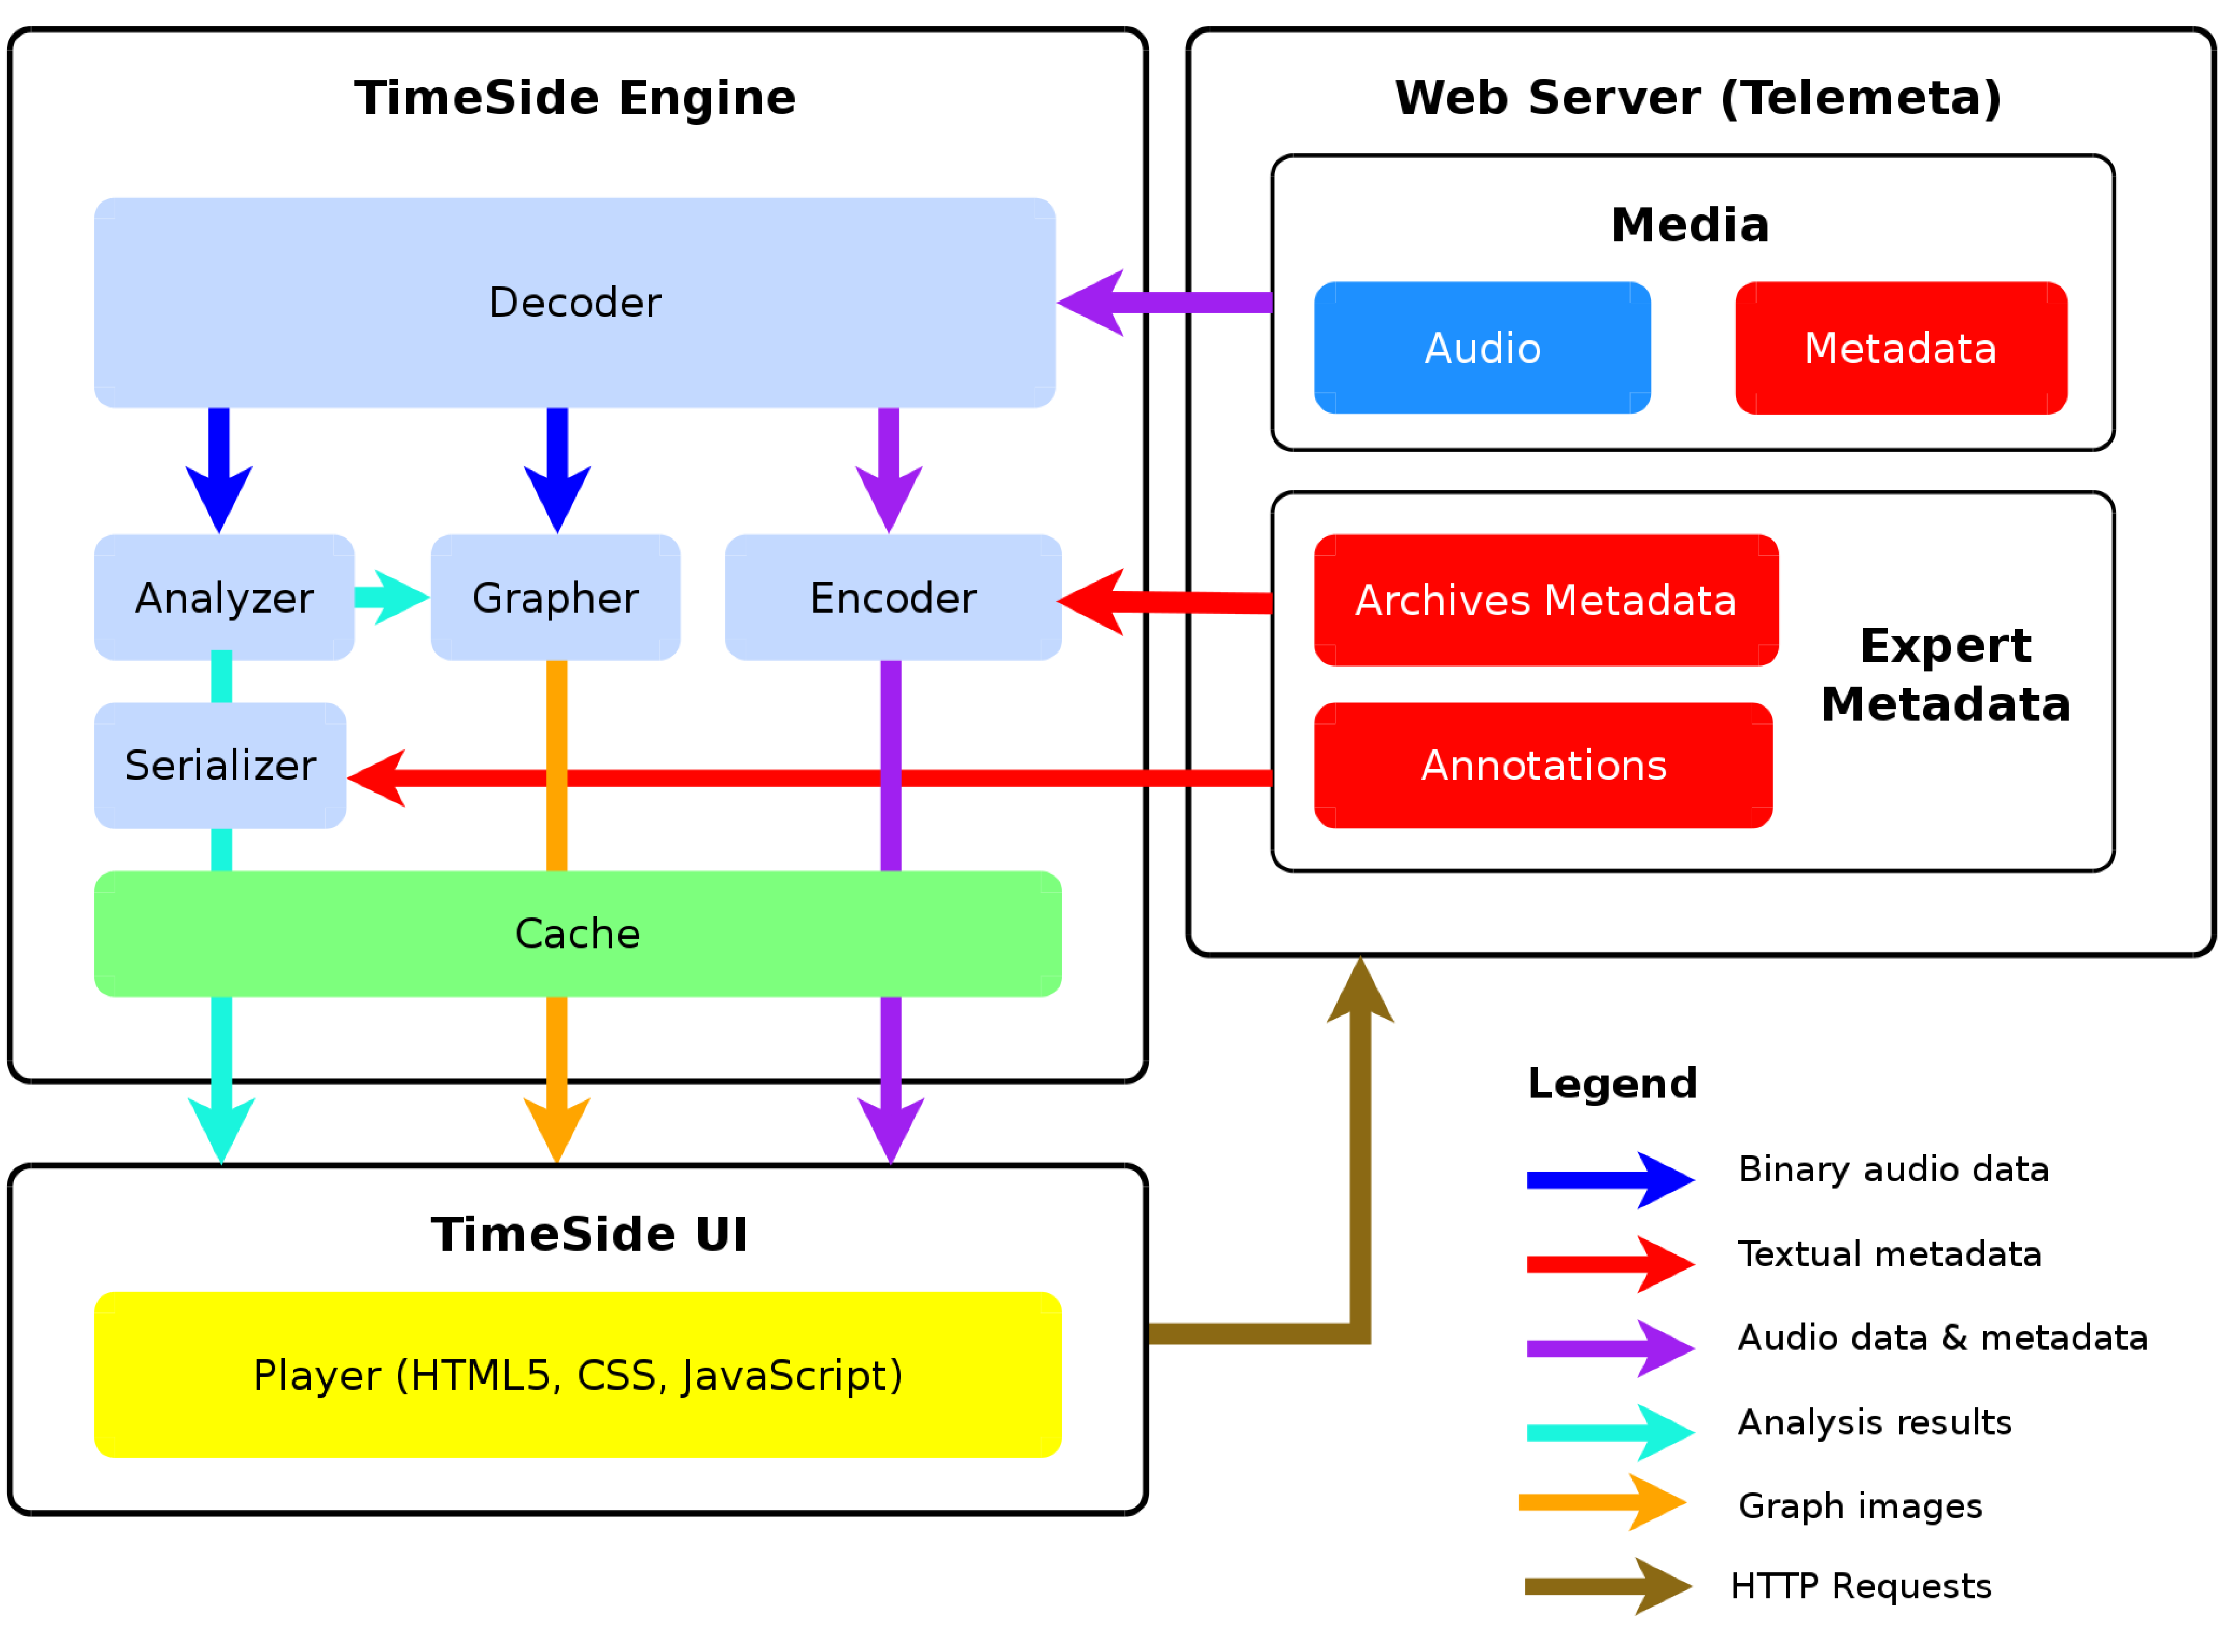
\includegraphics[width=0.7\linewidth]{img/timeside_schema_v3.pdf}
  \caption{TimeSide engine architecture and data flow with Telemeta web-server}\label{fig:TimeSide_Archi}
\end{figure*}


\subsection{Audio management}
TimeSide provides the following main features:
\begin{itemize}
\item Secure archiving, editing and publishing of audio files over
  internet.
\item Smart audio player with enhanced visualisation (waveform, spectrogram)
\item Multi-format support: reads all available audio and video formats  through Gstreamer, transcoding with smart streaming and caching methods% (FLAC, OGG, MP3, WAV and WebM)
  % \item \emph{Playlist management} for all users with CSV data export
\item "On the fly" audio analyzing, transcoding and metadata
    embedding based on an easy plugin architecture
\end{itemize}

\subsection{Audio features extraction}
In order to provide Music Information Retrieval analysis methods to be implemented over a large corpus for ethnomusicological studies, TimeSide incorporates some state-of-the-art audio feature extraction libraries such as Aubio\footnote{\url{http://aubio.org/}} \citep{brossierPhD}, Yaafe\footnote{\url{https://github.com/Yaafe/Yaafe}} \citep{yaafe_ISMIR2010} and Vamp plugins\footnote{ \url{http://www.vamp-plugins.org}}.

As a open-source framework and given its architecture and the flexibility provided by Python, the implementation of any audio and music analysis algorithm can be consider. Thus, it makes it a very convenient framework for researchers in computational ethnomusicology to develop and evaluate their algorithms.

Given the extracted features, every sound item in a given collection can be automatically analyze. The results of this analysis can be stored in a scientific file format like Numpy and HDF5 and serialized to the web browser through common markup languages: XML, JSON and YAML.


\subsection{Automatic Analysis of ethnomusicological sound archives}
Ongoing works lead by the DIADEMS project consist in implementing advanced classification, indexation, segmentation and  similarity analysis methods dedicated to ethnomusicological sound archives.

Besides music analysis, such automatic tools also deal with speech and noises classification and segmentation to enable a full annotation of the audio materials.

In the context of this project, both researchers from Ethnomusicological, Speech and Music Information Retrieval communities are working together to specified the tasks to be addressed by automatic analysis tools.

\section{Sound archives of the CNRS - Musée de l'Homme}\label{sec:archives-CREM}
Since June 2011, the Telemeta platform has been deployed to hold the \emph{Sound archives of the CNRS - Musée de l'Homme}\footnote{\url{http://archives.crem-cnrs.fr}} and is managed by the CREM (Center for Research in Ethnomusicology).
The platform aims to make these archives available to researchers and to the extent possible, the public, in compliance with the intellectual and moral rights of musicians and collectors.

\subsection{Archiving research materials}
The archives of CREM, the most important in Europe, are distinguished by their wealth:
\begin{itemize}
\item Nearly 3,500 hours of recordings of unpublished field.
\item Approximately 3700 hours of material published (more than 5000 discs, many of which are very rare).
\end{itemize}
The collection is sustained by the field missions of researchers on all continents. 

Through this platform, archivists can properly ensure the long-term preservation of data and continuously maintain and enrich the associated metadata.

Accessing the collections aid laboratory research, diachronic and synchronic comparisons, the preparation of new fieldwork and the training of PhD students.

Publishing collections also helps researchers making their work more visible. Besides making available and listenable the related corpora, researchers can also append related academic publications and provide temporal annotations to further illustrate their work.


\subsection{A collaborative platform}
Given the collaborative nature of the platform, both research and archivist can cooperate with colleagues to continuously enrich metadata associated to a sound item or a collection.  

Collaborative tools like markers and comments enable researchers from different institutions to work together on some common audio materials.
It also allows researchers to exchange data online with communities producing their music in their home countries.


\section{Conclusion}

The Telemeta open-source framework provides the researchers in musicology with a new platform to efficiently distribute, share and work on their research materials.
The platform has been deployed since 2011 to manage the \emph{Sound archives of the CNRS - Musée de l'Homme} which is the most important european collection of ethnomusicocological resources.

Furthermore, this platform is offered automatic music analysis capabilities through an external component, TimeSide that provides a flexible computational analysis engine together with web serialization and visualization capabilities. As an open-source framework TimeSide could be an appropriate platform for researchers in computational ethnomusicology to develop and evaluate their algorithms

Further works on the user interface will enhance the visualization experience with time and frequency zooming capabilities and will thus improve the accuracy and the quality of time-segment base annotations.


\section*{Acknowledgments} 
{\small The authors would like to thank all the people that have been involved in Telemeta specification and development or have provide useful input and feedback. 
The project has been partially funded by the French National Centre for Scientific Research (CNRS), the French Ministry of Culture and Communication, the TGE Adonis Consortium, and the Centre of Research in Ethnomusicology (CREM).}


%\bibliographystyle{plainnat}
\bibliography{fma2014_Telemeta}


\end{document}
